\documentclass[11pt,a4paper,twoside,openany]{book}

% PAQUETES ------------------------------------------------------------------------------
\usepackage[utf8]{inputenc}
\usepackage[spanish,es-tabla,es-nodecimaldot]{babel}
\usepackage{amsmath}
\usepackage{amsfonts}
\usepackage{amssymb}
% Manejo de simbolos de cita multiples
\usepackage{csquotes}
% Figuras
\usepackage{graphicx}
% Configuracion de interlineado (\onehalfspace y \singlespacing en capitulos)
\usepackage{setspace}
% Permite que las figuras floten en la posición en la que aparecen en el código
\usepackage{float}
% Permite dar estilo a los subtitulos de las figuras (captions)
\usepackage{caption}
% Permite sub-captions en sub-figuras (figuras dentro de figuras)
\usepackage{subcaption}
% Permite múltiples filas en tablas
\usepackage{multirow}
% Elimina numeracion de paginas en blanco
\usepackage{emptypage}
% Paquete para las figuras
\usepackage{wrapfig}
\usepackage{subcaption}
%Para cambiar la alineación predeterminada de una imagen de la izquierda o la derecha de una manera fácil
\usepackage[export]{adjustbox}
% Permite continuar con la numeración entre listas distintas
\usepackage{enumitem}
% Bibliografia
%\usepackage[
% 	backend=biber,
% 	style=numeric,
% 	sorting=none
% ]{biblatex}
%\addbibresource{./capitulos/bibliografia.bib}
% Introduce la bibliografía en el índice
\usepackage[nottoc]{tocbibind}
% Modificar encabezamientos y pie de páginas
\usepackage{fancyhdr}
% Rompe URLs largas
%\usepackage{breakurl}
% Soporte para estructuras de algoritmos en pseudocódigo
\usepackage[spanish,onelanguage,ruled,vlined,linesnumbered]{algorithm2e}
% Soporte de listado de codigo MATLAB
\usepackage[numbered,autolinebreaks]{mcode}
% Control de enlaces hipertexto en el documento. Este paquete debe cargarse el último.
\usepackage{hyperref}
% Configuracion interna del documento PDF, requiere hyperref
\hypersetup {
    pdfauthor = {AUTOR},
    pdfsubject = {TITULO},
    pdftitle = {Trabajo de Fin de Grado - Manual Técnico},
    pdfkeywords = {palabras, clave}
}
\graphicspath{{./img/}}

% Marca en rojo los elementos pendientes (TO-DOs)
\newcommand{\todo}[1]{\textcolor{red}{TODO: #1}}

% Informacion del documento -------------------------------------------------------------
\author{Antonio Ariza García y Enrique Gálan Gálan}
\title{IAA}
\date{LA FECHA}

% ESTILOS DE PAGINA ---------------------------------------------------------------------
% Indexación de contenidos hasta 3er nivel
\setcounter{tocdepth}{3}
\setcounter{secnumdepth}{3}
% Encabezado y pie de pagina
\pagestyle{fancy}
\fancyhf{}
\fancyhead[RO]{\rightmark}
\fancyhead[LE]{\leftmark}
\fancyfoot[LE,RO]{\thepage}
% Fijar altura vertical de la cabecera
\setlength{\headheight}{15pt}
% Lineas de encabezado y pie de pagina
\renewcommand{\headrulewidth}{2pt}
\renewcommand{\footrulewidth}{1pt}
% Interlineado de 1.5
\renewcommand{\baselinestretch}{1.5}
\renewcommand{\thesection}{\arabic{section}}
%Para renombrar figurename se debe hacer asi por el paquete idioma babel
\addto\captionsspanish{
  \renewcommand{\figurename}{Fig.}
  %\renewcommand{\chaptername}{Entregable}
}
%\renewcommand{\bibname}{Bibliografía}

% Enlaces
\hypersetup{
    colorlinks=true,
    urlcolor=cyan,
}
% Espacio despues de tablas
\setlength{\textfloatsep}{0.1cm}
\setlength{\parskip}{2pt}
\setlength{\parindent}{1em}

% DOCUMENTO ----------------------------------------------------------------------------
\begin{document}
\frontmatter

% PORTADA ---------------------------------------------------------------
\begin{titlepage}
\centering

\includegraphics[width=0.18\textwidth]{img/logo_uco_sin_texto.png}

\includegraphics[width=0.30\textwidth]{img/logo_uco_epsc.png}\par\vspace{1cm}
{\scshape\LARGE Universidad de Córdoba\par}
{\scshape\Large Escuela Politécnica Superior de Córdoba\par}
\vspace{1cm}
{\scshape\LARGE Ingeniería Informática\par}
{\scshape\Large Especialidad: Computación\par}
{\scshape\Large Cuarto curso. Primer cuatrimestre\par}
\vspace{1.5cm}
{\scshape\LARGE Introducción a los modelos computacionales.\par}
\vspace{1.5cm}
{\huge\bfseries Práctica 3: Redes neuronales de funciones de base radial.\par}
\vspace{1.2cm}
{\Large\itshape Antonio Ariza García\par}
DNI\par
\href{mailto:correo@uco.es}{i62argaa@uco.es}\par
\vfill

{\large Curso académico 2020-2021\\Córdoba, \today\par}
\end{titlepage}

% INDICES ---------------------------------------------------------------
%\pagenumbering{roman}
% Indice general
\tableofcontents
% Indice de figuras
\listoffigures
% Indice de tablas
%\listoftables

% DESARROLLO DE LA MEMORIA -------------------------------------------------------------
\mainmatter

% MANUAL TÉCNICO -----------------------------------------------------------------------
%\part{Prácticas} \label{part:practicas}
\section{Introducción} \label{ch:introduccion}

Este documento está realizado en Latex, forma parte de la asignatura Introducción al aprendizaje automático, de la escuela politécnica de Córdoba.
Es una breve introducción a Weka, software utilizado para aprendizaje automático y la minería de datos, está escrito en Java.
\newline
El siguiente documento tiene como objetivo presentarse como guión y entrega de prácticas, puede utilizarse como pequeña guía a la introducción a Weka y aprendizaje automático.
\chapter{Entregable 1}
\section{Transformación base de datos de la UCI (Machine learning repository) a formato .arff}

En este apartado veremos como transformar una base da datos del repositorio UCI al formato .arff.

\subsection{Base de datos Dermatology}

\begin{itemize}
\item Muchas de las bases de datos disponibles en la red se encuentran en formato .csv.
\item Además de usar ficheros .arff, Weka también permite usar ficheros .csv aunque hay que hacerlo con precaución.
\item Se pueden visualizar los ficheros con un editor de texto o mediante $ Tools \rightarrow ArffViewer $.
\end{itemize}

Una vez descargada la base de datos, la abrimos con excel. Entraremos en la opciones avanzadas en excel y cambiamos la configuración regional para que se utilice el ``.'' como separador decimal y la ``,'' como separador de miles. Una vez abierto el archivo, excel invoca el asistente de conversión de texto en el cual es importante resaltar la coma como separador de campos (Figura\ref{fig:asistente_excel}). Guardamos el fichero con formato nativo xls para tenerlos para futuras modificaciones y también lo guardamos como formato csv que si lo puede leer Weka.

\begin{figure}[H]
	\centering
    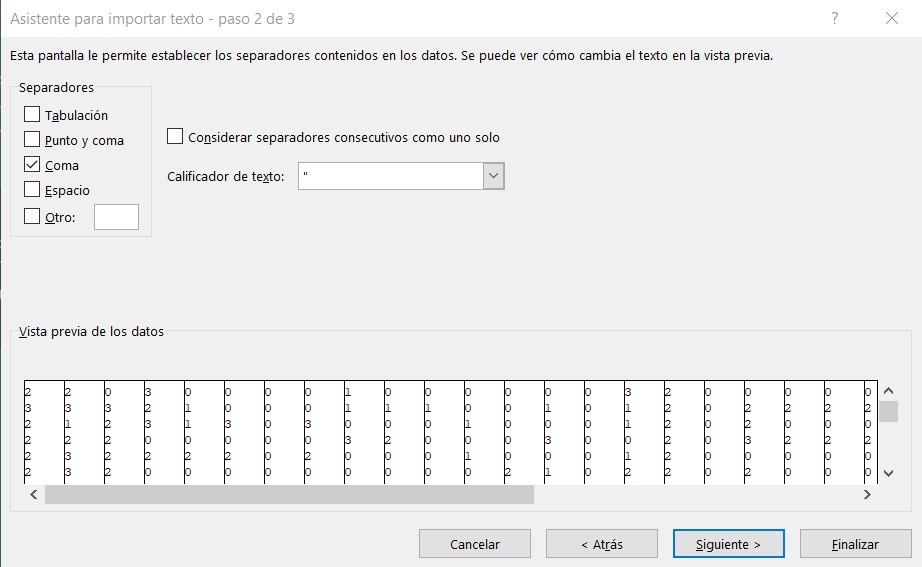
\includegraphics[width=\textwidth, height=1.05\textwidth]{asistente_conversion_excel}
    \caption{Asistente conversión Excel}
    \label{fig:asistente_excel}
\end{figure}

Abrimos weka, elegimos ``csv'' como tipo de archivo y muy importante seleccionar la opción ``invoke''. (Figura\ref{fig:invoke}).
Se nos abrirá el convertidor de Weka (Figura\ref{fig:conversor_weka}) en donde debemos cambiar algunos parámetros.
 
\begin{figure}[H]
    \centering
    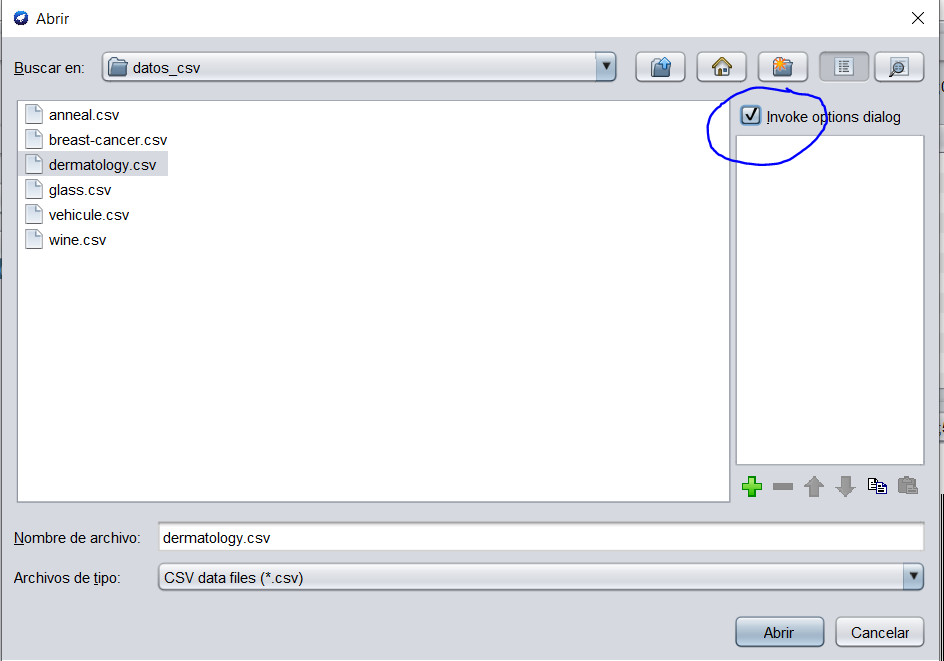
\includegraphics[width=\textwidth, height=1.15\textwidth]{weka_invoke}
    \caption{Abrir archivo en weka}
    \label{fig:invoke}
\end{figure}

\begin{figure}[H]
    \centering
    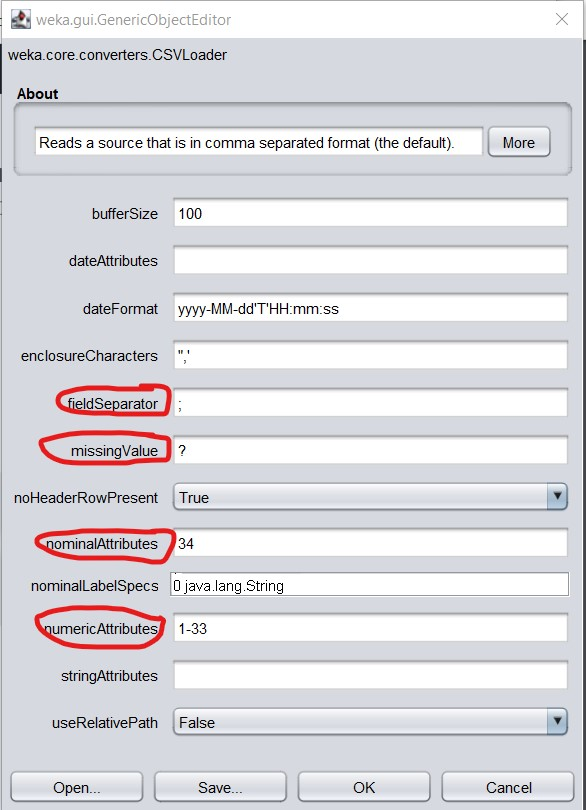
\includegraphics[width=0.7\textwidth]{Weka_convertidor}
    \caption{Convertidor Weka}
    \label{fig:conversor_weka}
\end{figure}

\begin{itemize}
\item FielSeparator: Separador de campos que será ``;''.
\item MissingValue: Carácter que usaremos para valores perdidos.
\item NoHeaderRowPresent: Decimos si el fichero no trae una fila al principio con los nombres de las variables. (En nuestro caso no la trae, decimos True).
\item NominalAttributes: Lista de variables nominales.
\item NumericAttributes: Lista de variables numéricas. (Se pueden poner rangos, ej:1-3,10-33).
\end{itemize}

Al aceptar comprobamos que nos dá un error (Figura\ref{fig:fallo}), hay problemas con la versión de Weka, por lo tanto he optado a a cambiar el fichero a mano. Para cambiar los ``;'' es mejor hacerlo con un editor de texto como Atom o Sublime Text, dandole a la tecla Control + F se abre el buscador y nos permite reemplezar todos los ``;'' por ``,'' (con esto evitamos hacerlo uno a uno) ya que Weka utiliza la coma para la separación entre los datos. En la siguiente Figura podemos ver el aspecto de los datos del fichero .arff (Figura\ref{fig:atributos}), es necesario saber de que tipo son las variables(numérica o nominal) que tenemos en la base de datos y escribirlo al principio de nuestro fichero, basta con mirar en la página UCI. (Figura\ref{fig:datos}). Por ejemplo elegimos la base de datos Dermatology (\url{https://archive.ics.uci.edu/ml/datasets/Dermatology}), pinchamos en ``Data Set Description'' y se nos descargará un fichero descriptivo sobre la base de datos, en el cual encontramos una descripción sobre la misma, número de atributos y tipo, número de instancias, clases. 

Vemos que la última columna es la clase a predecir (variable dependiente), con 5 clases distintas (1,2,3,4,5 o U). 
Los valores perdidos se representan con ``?'' y los valores no aplicables con ``-'' (y deben considerarse como categoría).

\begin{figure}[H]
    \centering
    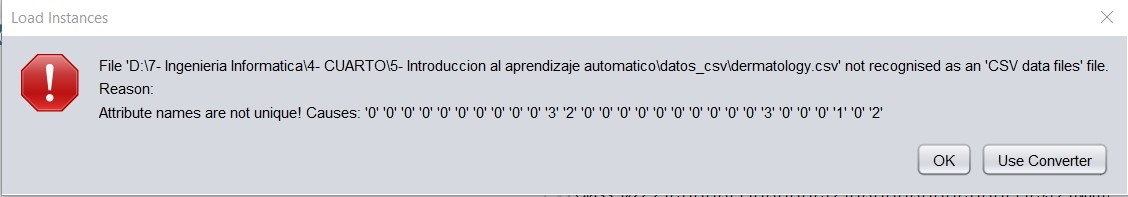
\includegraphics[width=\textwidth, height=0.35\textwidth]{error}
    \caption{Fallo del convertidor}
    \label{fig:fallo}
\end{figure}

\begin{figure}[H]
	\begin{subfigure}[H]{0.48\textwidth}
    	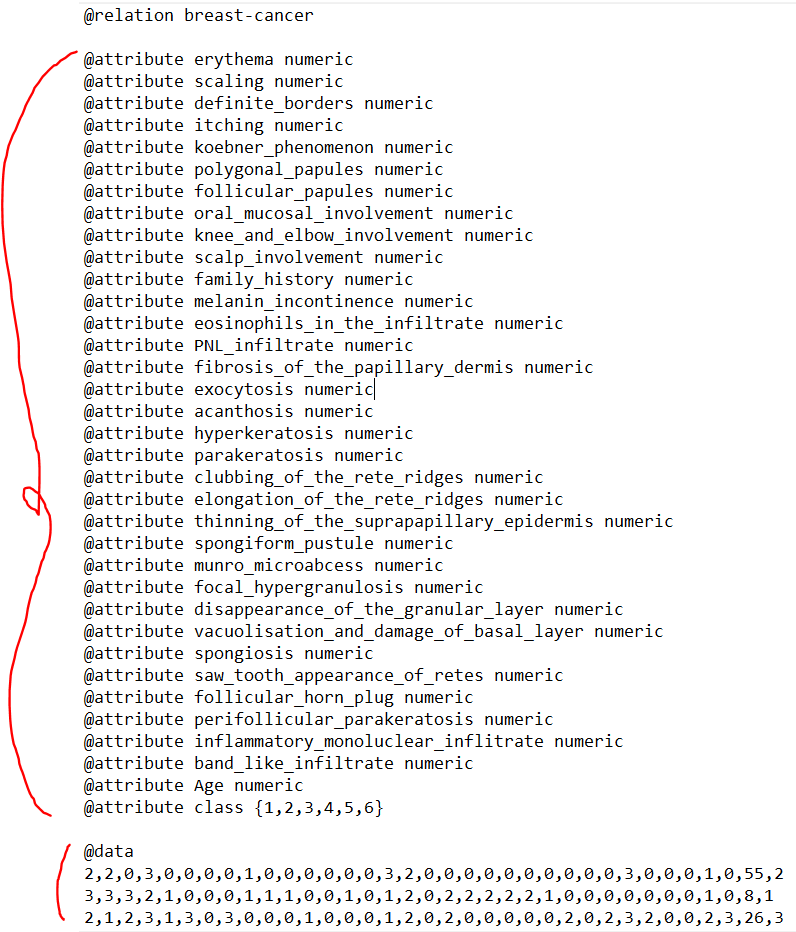
\includegraphics[width=\linewidth, height=1.5\linewidth, left]{fichero_arff}	
    	\caption{Inicio fichero}
    	\label{fig:datos}
	\end{subfigure}
	\hfill
	\begin{subfigure}[H]{0.48\textwidth}
    	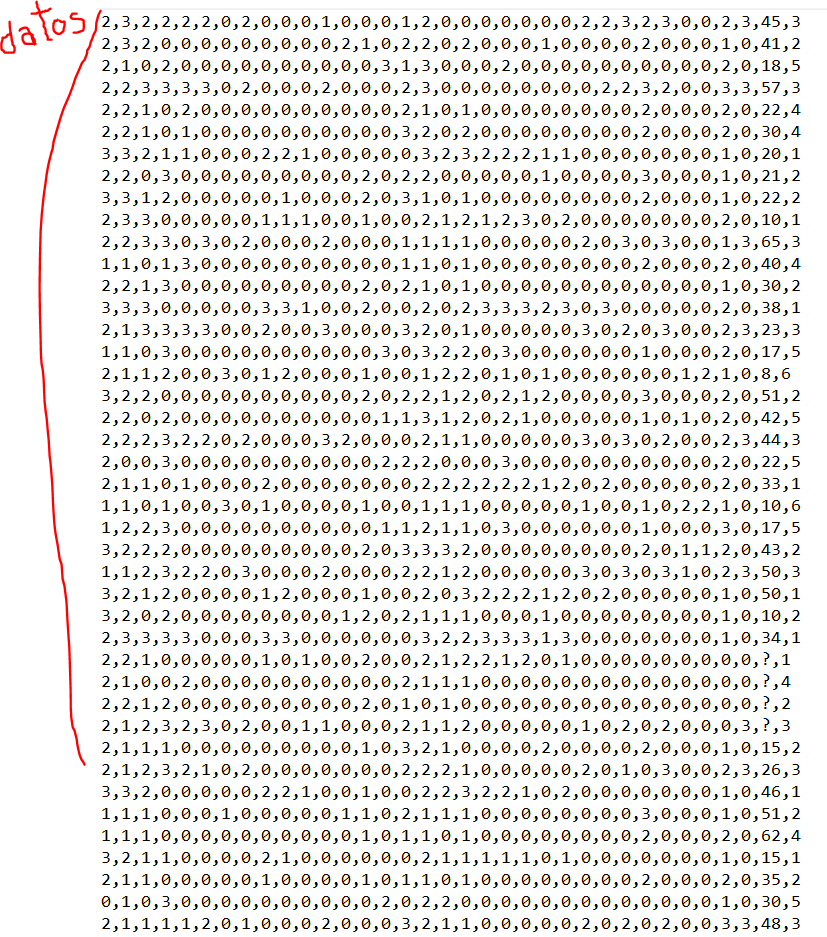
\includegraphics[width=\linewidth, height=1.5\linewidth, left]{fichero_arff2}	
    	\caption{Final fichero}
    	\label{fig:atributos}
	\end{subfigure}
	\caption{Aspecto Fichero .arff}
	\label{fig:fichero_arff}
\end{figure}

Para todas las bases de datos he realizado el mismo procedimiento:
\begin{itemize}
\item \url{https://archive.ics.uci.edu/ml/datasets/Breast+Cancer}
\item \url{https://archive.ics.uci.edu/ml/datasets/Glass+Identification}
\item \url{https://archive.ics.uci.edu/ml/datasets/Statlog+%28Vehicle+Silhouettes%29}
\item \url{https://archive.ics.uci.edu/ml/datasets/Wine}
\item \url{https://archive.ics.uci.edu/ml/datasets/Zoo}
\end{itemize}

%------------------------------------------------------------------------
%-------------------------------------------------------------------------
\newpage
\section{Filtros en Weka}

Weka permite aplicar una gran diversidad de filtros sobre los datos, permitiendo realizar transformaciones sobre ellos de todo tipo.

\begin{itemize}
	\item No tienen en cuenta el último atributo del dataset a la hora de hacer un tratamiento sobre los datos.
	\item Por defecto toman el último atributo como clase o valor numérico de salida para regresión, aplicándose el filtro a todos los patrones y atributos.
	\subitem Opción Ignore Class = false
	\item Si queremos cargar una serie de datos a los que aplicar filtros en su totalidad, indicarlo en la opción correspondiente en el filtro.
	\subitem Opción Ignore Class = true
\end{itemize}

\subsection{Base de datos audiology}
Cargue la base de datos auidiology. Pruebe todas las combinaciones posibles para pasar los atributos nominales a binarios, según los detalles proporcionados en la transparencia numero 8, mostrando en cada caso un ejemplo de cómo quedarían los nominales con 2 valores y con 3 o más valores usando esas combinaciones.
\begin{itemize}
    \item BinaryAttributesNominal=False
    \begin{figure}[H]
    \centering
    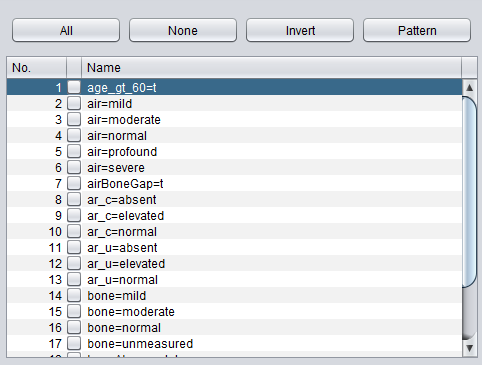
\includegraphics[width=\textwidth]{img/BAN=False.PNG}
    \caption{BinaryAttributesNominal=False}
\end{figure}

Como vemos en la figura superior, los atributos nominales con dos etiquetas como es el caso de "agegt60" se ha transformado en un solo atributo binario cuyo nombre coincide con el de una de sus etiquetas en este caso t(true) quedando con el nombre de "agegt60=t", aquellos que en este atributo posean un valor de 1 significara que tienen un valor true, para el atributo anterior, sin embargo aquellos que tengan un valor de 0 tendrían un valor de false.
Muy distinto es el caso de los atributos nominales que poseen tres o más etiquetas como es el caso del atributo air, que posee hasta cinco etiquetas, en este caso se crea un atributo para cada etiqueta indicando en cada caso con uno o cero la presencia o no de este atributo.
\end{itemize}

\begin{itemize}
    \item TransformAllValues=True
    \begin{figure}[H]
    \centering
    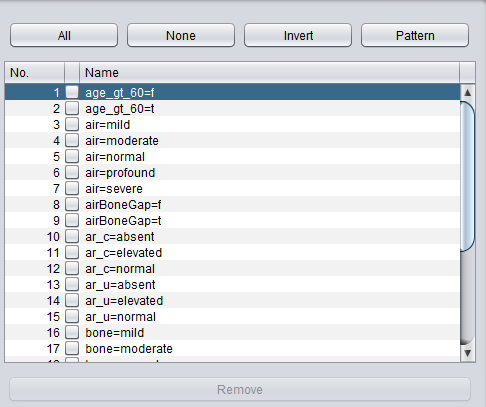
\includegraphics[width=\textwidth]{img/TAV=True.PNG}
    \caption{TransformAllValues=True}
    
\end{figure}
En este último caso vemos que tanto aquellos atributos con dos etiquetas(agegt60) que poseían las etiquetas t(true) y f(false) han sido transformados a dos atributos binarios, uno con valor de true y otro con valor de false indicando con uno o cero la presencia o no del mismo, de igual modo aquellos con tres o mas etiquetas quedan como lo hemos visto antes transformándose en tantos atributos binarios como etiquetas tuviera el atributo nominal.
\end{itemize}

\subsection{Tres filtros no supervisados}
Elija tres filtros no supervisados de los que aparecen listados, explíquelos y describa como quedan los datos antes y después al aplicarlos sobre una o varias bases de daros de las indicadas en moodle ya en formato .arff
\begin{itemize}
    \item Normalize: Normaliza todos los datos de manera que el rango de los datos pase a ser [0,1].Para normalizar un vector se utiliza la fórmula:
$$ X(i) = \dfrac{x(i)}{ \sqrt{\sum_{i=1}^{n} x(i)^2}} $$

En este caso lo vamos a aplicar a nuestra base de datos iris.arff que posee cuatro atributos numéricos y un atributo clasificador.
\begin{figure}[H]
    \centering
    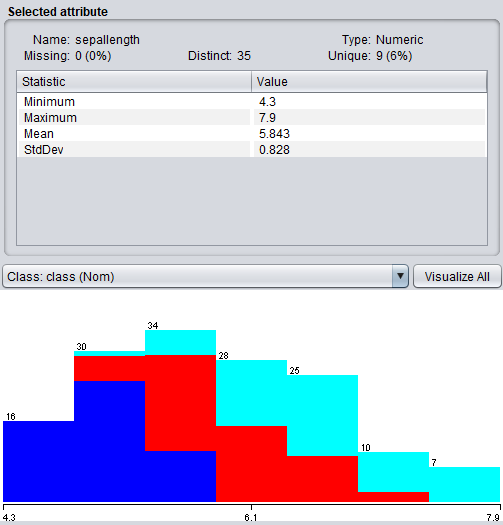
\includegraphics[width=\textwidth]{img/BN.PNG}
    \caption{Antes de aplicar filtro Normalize}
    
\end{figure}

Como vemos en la figura superior, en la cual aún no hemos aplicado el filtro Normalize, el atributo sepallenght de tipo numérico nos muestra como se encuentra repartidos los valores en función de su clase, pero siempre en un rango de entre 4,3 y 7,9. Sin embargo una vez aplicado el filtro Normalize este rango quedará normalizado entre los valores 0 y 1.
\begin{figure}[H]
    \centering
    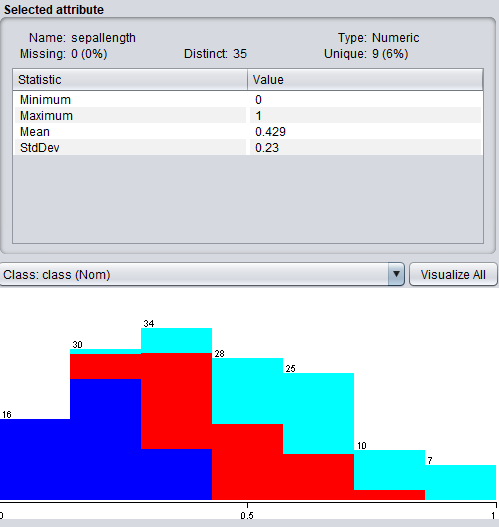
\includegraphics[width=\textwidth]{img/AN.PNG}
    \caption{Después de aplicar filtro Normalize}
\end{figure}

    \item Remove: Borra un conjunto de atributos del fichero de datos, para ello debemos de indicarle el índice de los atributos que queremos borrar de nuestro fichero de datos. A continuación se indica como hacerlo:
    \begin{figure}[H]
    \centering
    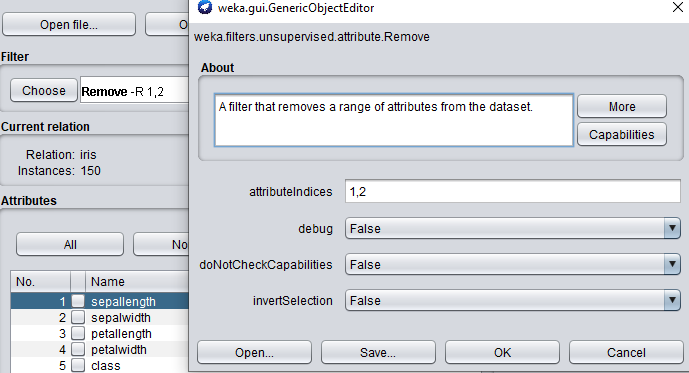
\includegraphics[width=\textwidth, height=0.7\textwidth]{img/Rem.PNG}
    \caption{Indicaciones del filtro Remove}
    \label{fig:filtro_remove}
\end{figure}

Es en el apartado ``attributeIndices'' donde indicamos los índices de los atributos que queremos borrar, podemos indicar los índices que queremos borrar o bien separados por comas o bien separados por guión lo que indicara que queremos borrar un rango de atributos.

    \item ReplaceMissingValues:
Reemplaza todos los valores indefinidos por la moda en el caso de que
sea un atributo nominal o la media aritmética si es un atributo numérico.
Para este caso hemos cogido el fichero de datos iris.arff y lo hemos modificado eliminando tres de sus valores como aparece a continuación.
 \begin{figure}[H]
    \centering
    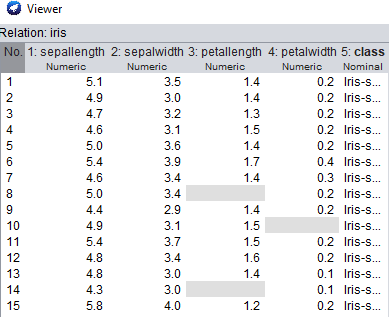
\includegraphics[width=\textwidth, height=1.1\textwidth]{img/BRP.PNG}
    \caption{Fichero con valores desconocidos}
    \label{fig:ReplaceMissingValues}
\end{figure}

En la siguiente figura se muestra como al aplicar el filtro ReplaceMissingValues los valores se han sustiudo por la media de cada atributo ya que ambos son numéricos.
 \begin{figure}[H]
    \centering
    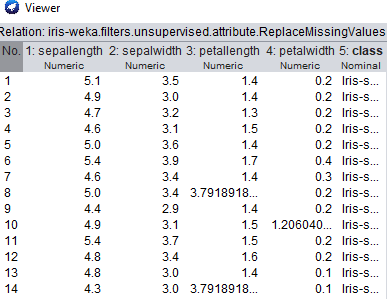
\includegraphics[width=\textwidth]{img/ARP.PNG}
    \caption{Aplicación del filtro ReplaceMissingValues}
\end{figure}

\end{itemize}

\subsection{Tres filtros supervisados}

Elija tres filtros no supervisados de los que aparecen listados, explíquelos y describa como quedan los datos antes y después al aplicarlos sobre una o varias bases de daros de las indicadas en moodle ya en formato .arff
\begin{itemize}
    \item Resample: Produce una submuestra aleatoria de un conjunto de datos utilizando muestreo con reemplazo o sin reemplazo.
El conjunto de datos original debe caber completamente en la memoria. Se puede especificar el número de instancias en el conjunto de datos generado. El conjunto de datos debe tener un atributo de clase nominal. De lo contrario, use la versión sin supervisión. El filtro se puede hacer para mantener la distribución de la clase en la submuestra o para sesgar la distribución de la clase hacia una distribución uniforme.
 \begin{figure}[H]
    \centering
    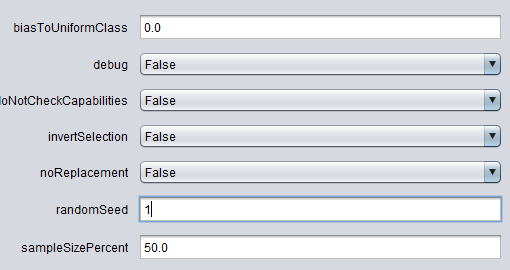
\includegraphics[width=\textwidth, height=0.8\textwidth]{img/opc_resample.PNG}
    \caption{Opciones del filtro Resample}
\end{figure}
Como vemos en la figura de arriba estas son las distintas opciones que nos plantea el filtro Resample, en este caso en particular hemos decidido el generar una nueva muestra aleatoria que siguiera la misma distribución que los datos de entrada y además tal como vemos en la ultima opción sampleSizePercent en la cual indicamos un cincuenta, esto quiere decir que el tamaño de nuestra muestra generada será del cincuenta por ciento de nuestra muestra inicial.En la siguiente figura mostramos los resultados de su aplicación.
 \begin{figure}[H]
    \centering
    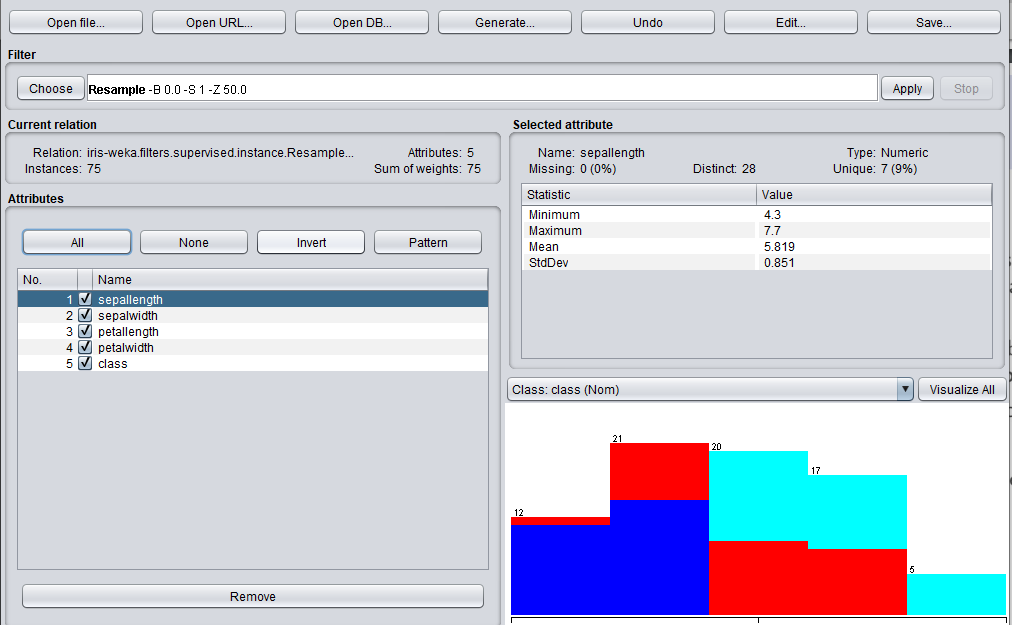
\includegraphics[width=\textwidth]{img/resample.PNG}
    \caption{Resultado de aplicar el filtro Resample}
\end{figure}
    \item SpreadSubsample: Produce una submuestra aleatoria de un conjunto de datos. El conjunto de datos original debe caber completamente en la memoria. Este filtro le permite especificar la "dispersión" máxima entre la clase más rara y la más común. Por ejemplo, puede especificar que haya como máximo una diferencia de 2: 1 en las frecuencias de clase. Cuando se usa en modo por lotes, los lotes posteriores NO se vuelven a muestrear.
    \item Discretize: Discretiza un conjunto de valores numéricos en rangos de datos. Como parámetros
    toma los índices de los atributos discretizar (attribute indices) y el número de particiones en que queremos que divida los datos (bins). Si queremos que las particiones las realice por la frecuencia de los datos y no por el tamaño de estas tenemos la opción useEqualFrecuency. Si tenemos activa esta última opción podemos variar el peso de las instancias para la definición de los intervalos con la opción DesiredWeightOfInstancesPerInterval. Si, al contrario tenemos en cuenta el número de instancias para la creación de intervalos podemos usar findNumBins que optimiza el procedimiento de confección de los mismos. Otras opciones son makeBinary que convierte los atributos en binario e invertSelection
    que invierte el rango de los atributos elegidos.
\end{itemize}



 



\chapter{Entregable 2}

\begin{itemize}
	\item El preprocesamiento es uno de los procesos más importantes en el flujo de acciones sobre un conjunto de datos. Es determinante para la obtención de modelos con buen rendimiento.
	\item Cada conjunto de datos necesita un preprocesamiento concreto diferente del realizado a otros.
\end{itemize}

\section{Preprocesamiento conjunto de datos de altura de ola}

Describa las operaciones de procesamiento que ha realizado sobre la base de datos proporcionada y como queda la base de datos al final ya procesada.

\subsection{Atributos TIDE, VIS, MWD}
Eliminaremos aquellos atributos que tengan más del 40\% de datos perdidos.
Como podemos comprobar los atributos TIDE, VIS, MWD no aportan nada a nuestro modelo, ya que todos sus valores son nulos. Eliminaremos estos tres atributos de la base de datos, quedándonos con los 15 restantes. Podemos utilizar el filtro Remove explicado en el capitulo anterior. (\ref{fig:filtro_remove})

%En nuestro caso no es necesario cambiar los atributos nominales a binarios, puesto que todos son numericos. 

El atributo DEWP tiene 33\% de los valores perdidos (\ref{fig:DEWP_missing}), por lo tanto también hemos decidido eliminarlo, pues tendríamos que reemplazar todos esos valores por la media e insertaríamos muchos datos iguales en la base de datos.

\begin{figure}[H]
	\centering
	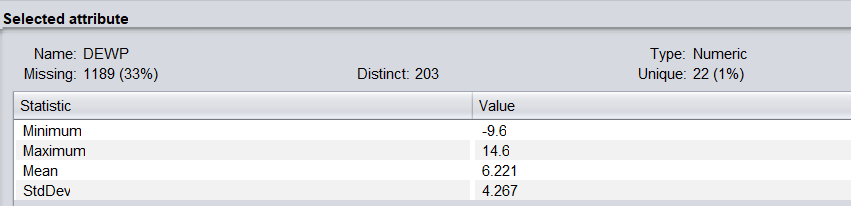
\includegraphics[width=\textwidth, height=0.35\textwidth]{DEWP_missing}
    \caption{DEWP Datos perdidos}
    \label{fig:DEWP_missing}
\end{figure}

\subsection{Recuperación de datos perdidos}

Existen muchas técnicas para la recuperación de datos perdidos.
\begin{itemize}
	\item Reemplazar por la media del conjunto de datos. También se puede reemplazar por la mediana o la moda dependiendo del tipo de atributo. Es un poco más justa cuando se emplean patrones de la misma clase.
	\item Regresión entre atributos (sin datos perdidos).
	\item Mediante técnicas de Machine Learning.
\end{itemize}
\newpage

\begin{wrapfigure}{l}{0.36\textwidth}
	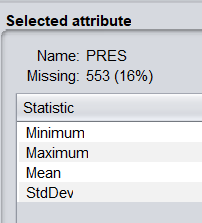
\includegraphics[width=0.9\linewidth, height=5cm]{PRES_1}
	\caption{Atributo PRES}
	\label{fig:PRES}
\end{wrapfigure}

El atributo PRES tiene el 16\% de datos perdidos (Fig\ref{fig:PRES}). 
En nuestro caso hemos utilizado el reemplazo por la media, para hacer esto utilizamos el filtro ``ReplaceMissingValues'' explicado en el capítulo anterior, (Fig\ref{fig:ReplaceMissingValues}) este filtro no calcula la media dependiendo del atributo clase si no que le asigna la misma media a todos. Al utilizar el filtro veremos como el porcentaje ``Missing'' se pone a 0\%.

\subsection{Selección de atributos}

Consiste en obtener una representación reducida del conjunto de datos que preserve información importante de la base de datos. Objetivos: 

\begin{itemize}
	\item Reducir la complejidad del problema eliminando atributos irrelevantes o redundantes.
	\item Aumentar el rendimiento de los modelos.
	\item Acelerar el proceso de aprendizaje.
	\item Reducción del sobreajuste.
\end{itemize}

Aunque en Weka hay muchas formas de seleccionar atributos (como análisis de correlaciones), nos centraremos en el método mediante búsqueda + evaluación. Seleccionamos como: $ ``Attribute evaluator'' \rightarrow CfsSubsetEval$ y como $ ``Search Method'' \rightarrow BestFirst $  
En la (Figura\ref{fig:Seleccion_atributos}) comprobamos como nos selecciona los atributos 2,4,5,7,8,9,10,11,12.

\begin{figure}[H]
	\centering
	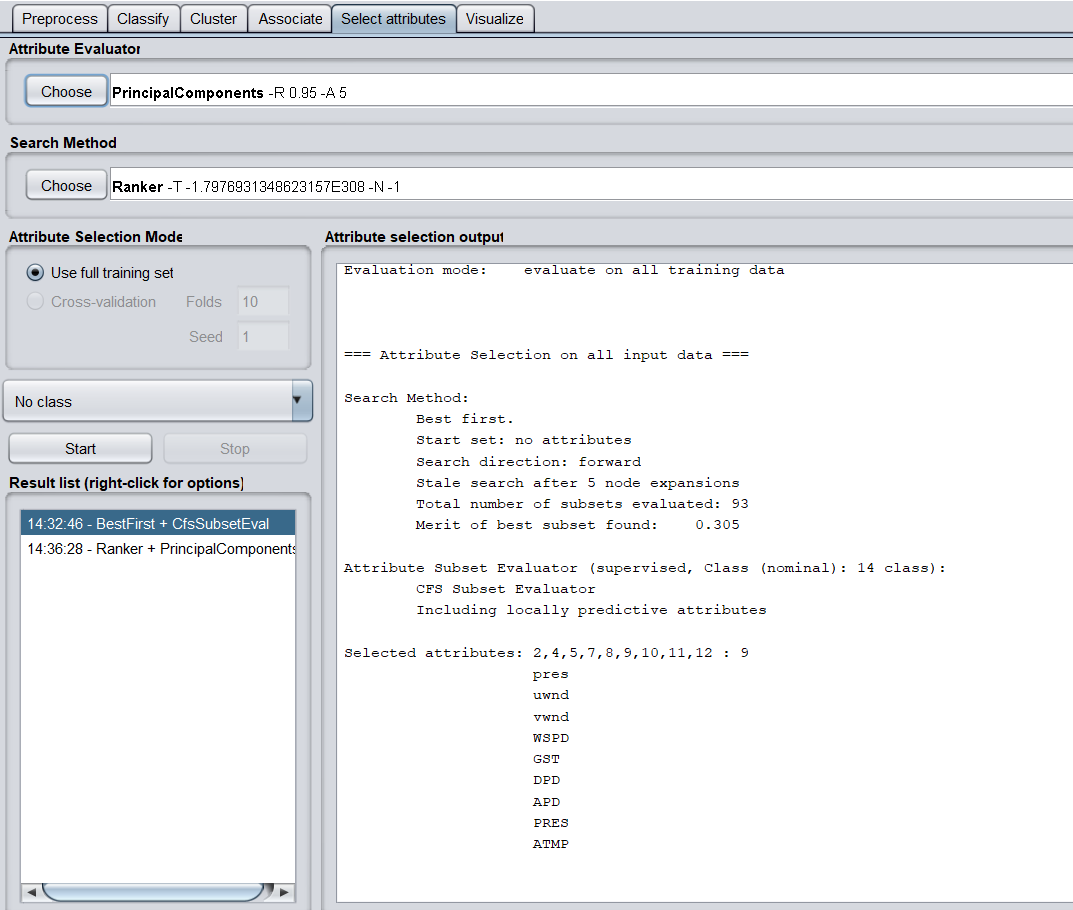
\includegraphics[width=\textwidth, height=\textwidth]{Seleccion_atributos}
    \caption{Seleccion de atributos}
    \label{fig:Seleccion_atributos}
\end{figure}

Volviendo a nuestro conjunto de entrenamiento procedemos a utilizar el filtro ``Remove'' para dejar solo los atributos indicados, para ellos copiamos y pegamos los atributos e invertimos la selección para que nos elimine los no seleccionados (en este caso eliminaremos los atributos AIR, RHUM, WDIR, WTMP). Una vez tenemos los atributos procedemos a realizar un experimento con un clasificador ``Logistic'' y la configuración por defecto para comprobar si hemos mejorado el rendimiento y los atributos eliminados no aportaban mucha información. (\ref{fig:Logistic_rendimiento})

\begin{figure}[H]
	\begin{subfigure}[H]{\textwidth}
    	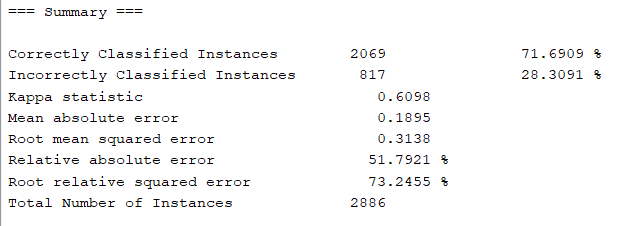
\includegraphics[width=\linewidth]{logistic_1}	
    	\caption{Antes}
	\end{subfigure}
	\hfill
	\begin{subfigure}[H]{\textwidth}
    	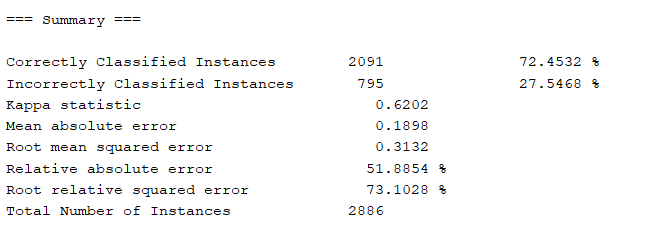
\includegraphics[width=\linewidth]{logistic_select}	
    	\caption{Despues}
   
	\end{subfigure}
	\caption{Logistic rendimiento}
	\label{fig:Logistic_rendimiento}
\end{figure}

\subsection{Correlación}

El rendimiento de algunos algoritmos puede deteriorarse si dos o más variables están estrechamente relacionadas. Eliminar algunas de las variables pueden mejorar el rendimiento del modelo.
Para obtener la matriz de correlaciones nos situamos en la pestaña de selección de atributos y seleccionamos como: $ ``Attribute evaluator'' \rightarrow PrincipalComponents$ y como $ ``Search Method'' \rightarrow Ranked $

\begin{table}[H]
	\resizebox{1.07\textwidth}{!}{
	\begin{tabular}{|l|c|c|c|c|c|c|c|c|c|}
	\hline
	& pres & uwnd & vwnd & WSPD & GST & DPD & APD & PRES & ATMP \\ \hline
	pres & 1 & 0.14 & -0.2 & -0.34 & -0.37 & -0.26 & -0.43 & 0.93 & 0.26 \\
	uwnd & 0.14 & 1 & -0.17 & -0.07 & -0.17 & -0 & -0.03 & 0.05 & 0.17 \\
	vwnd & -0.2 & -0.17 & 1 & 0.31 & 0.31 & 0.07 & 0.13 & -0.18 & -0.01 \\
	WSPD & -0.34 & -0.07 & 0.31 & 1 & \color{red}0.99 & 0.01 & 0.1 & -0.31 & -0.17 \\
	GST & -0.37 & -0.07 & 0.31 & 0.99 & 1 & 0.04 & 0.14 & -0.34 & -0.2 \\ 
	DPD & -0.26 & -0 & 0.07 & 0.01 & 0.04 & 1 & 0.71 & -0.27 & -0.33  \\
	APD & -0.43 & -0.03 & 0.13 & 0.1 & 0.14 & 0.71 & 1 & -0.44 & -0.44 \\
	PRES & 0.93 & 0.05 & -0.18 & -0.31 & -0.34 & -0.27 & -0.44 & 1 & 0.28 \\
	ATMP & 0.26 & 0.17 & -0.01 & -0.17 & -0.2 & -0.33 & -0.44 & 0.28 & 1\\
	\hline
	\end{tabular}
	}
	\caption{Matriz de correlación}
	\label{tabla:Matrizcorrelacion}
\end{table}

Comprobando la matriz de correlación (Tabla\ref{tabla:Matrizcorrelacion} nos damos cuenta como existe una relación entre el atributo GST y WSPD. Mirando el resto de los atributos hemos decidido eliminar el atributo WSPD, debemos tener cuidado porque este análisis puede llevar a ilusiones o relaciones falsas. Eliminaremos el atributo y haremos algunas pruebas con el conjunto de test en el cual también debemos eliminar los mismos atributos que en el conjunto de entrenamiento (Mirar el siguiente punto relacionado con el conjunto de test). Al realizar las pruebas obtenemos un 72,35\% de acierto en clasificación, anteriormente obtuvimos un 72,45\%, aunque hemos perdido 0,1 es señal de que las variable están relacionadas y no aportan mucho al conjunto de datos. Continuando con este procedimiento y obteniendo otra vez la matriz de correlaciones podemos continuar eliminando algunos atributos más. En nuestro caso hemos eliminado: 
\begin{itemize}
	\item WSPD
	\item PRES
	\item uwnd
\end{itemize} 

\section{Preprocesamiento conjunto Test}

El proceso de procesamiento del conjunto test es prácticamente similar al del conjunto de entrenamiento, con algunas pequeñas diferencias, variando únicamente el proceso de normalización de atributos y el reemplazamiento de los atributos perdidos.

\subsection{Tratamiento de atributos}
Todos los atributos eliminados en el conjunto de datos de entrenamiento deben ser eliminados también en el conjunto de test, tanto los eliminados al principio como los eliminados en el proceso de selección de atributos. También hay que reemplazar los datos perdidos como hicimos con el atributo PRES por ejemplo, este reemplazamiento debe ser por los valores usados en train (podemos hacer uso del filtro ``ReplaceMissingWithUserConstant'').

\subsection{Normalización}
%En nuestro caso no hemos normalizado, pero si fuera necesario.
Para normalizar los datos del conjunto de test debemos obtener todos los mínimos y máximos de cada atributo que podemos ver pinchando encima de cada uno o en el botón de Edit. Una vez tengamos todos los valores debemos utilizar el filtro ``MathExpression''.
En expresión debemos introducir los mínimos y máximos tal como aparece en \ref{fig:Normalizacion}, en ``ignoreRange'' se indicará el índice del atributo, y en ``invertSelection'' lo seleccionaremos en true para que solo realice la normalización del atributo indicado. Este proceso debe realizarse para cada unos de los atributos, indicando para cada uno sus correspondientes valores mínimos y máximos.

\begin{figure}[H]
	\centering
	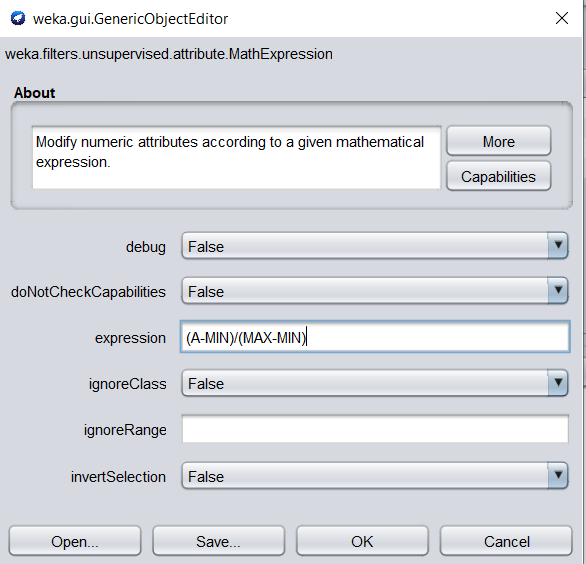
\includegraphics[width=\textwidth]{normalizacion}
    \caption{Filtro Normalizacion}
    \label{fig:Normalizacion}
\end{figure}






\chapter{Entregable 3}

\section{Base de datos WINE}

Escoja una de las bases de datos de la clasificación para el trabajo de las dispuestas en Moodle.Aplique el preprocesamiento adicional (si se puede aplicar) sobre: 1) reemplazamiento de datos perdidos, 2) normalización y 3) paso de nominal a binario u ordinal a numérico.
Explique el procesamiento que haya llevado a cabo en los aspectos citados, y de no tener que hacerlo expliqué también el por qué.

Nuestro ejemplo elegido en este caso que ha sido wine.arff solo hemos tenido que normalizar los datos ya que no teníamos ningún dato perdido y además todos los atributos de nuestro fichero eran numéricos por lo que nos ha sido bastante sencillo.
\begin{figure}[H]
    \centering
    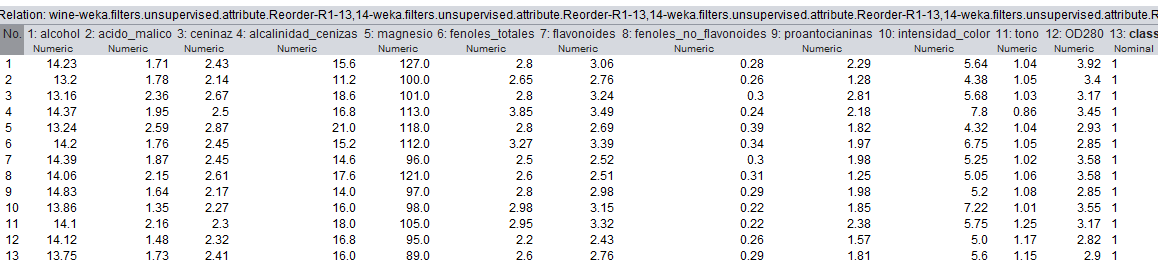
\includegraphics[width=\textwidth]{img/BNorm.PNG}
    \caption{Wine.arff antes de aplicar el filtro Normalize}
\end{figure}
Como vemos en la figura anterior los valores originales de nuestro fichero están sin organizar por lo tanton aplicaremos el filtro para conseguir que todos queden entre cero y uno.
\begin{figure}[H]
    \centering
    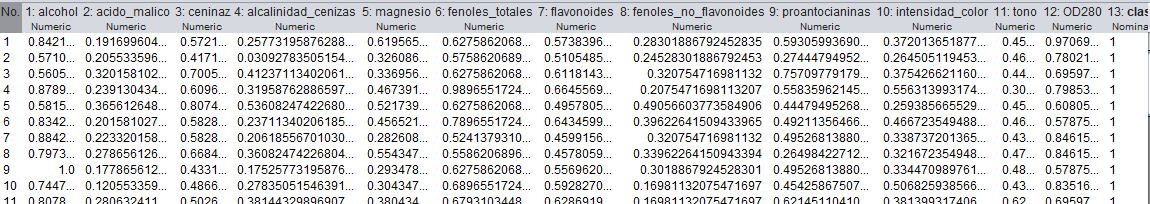
\includegraphics[width=\textwidth]{img/ANorm.PNG}
    \caption{Wine.arff una vez normalizado}
\end{figure}


\subsection{Algoritmo clasificación KNN}
Con la base de datos escogida anteriormente, use el algoritmo de clasificación KNN con un 10-fold crossvalidation. Use un valor de vecinos k=3 dejando por defecto el resto de parámetros.

Para realizar este ejercicio una vez ya tenemos preprocesada nuestra base de datos, nos vamos al apartado classify dentro de Weka, una vez aquí escogemos nuestro clasificador deseado, en este caso vamos a utilizar el clasificador KNN, conocido como algoritmo del vecino más cercano, para ello debemos de entrar dentro de la carpeta lazy en el cual se encuentra y seleccionar el clasificador ibk que es el nombre asignado en Weka para nuestro algoritmo. Una vez seleccionado debemos de modificar algunos valores por defecto ya que por defecto el numero de vecinos con el que comparar en uno es decir k=1, para nuestro problema en concreto tal y como nos indica en el enunciado debemos de cambiarlo y usar k=3, y además utilizar crossvalidation con 10 folds tal y como se muestra en la figura de abajo.

\begin{figure}[H]
    \centering
    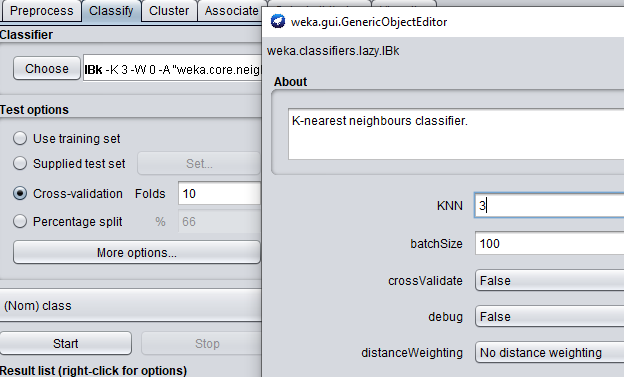
\includegraphics[width=\textwidth]{img/IB3.PNG}
    \caption{Valores modificados para IBK, k=3}
\end{figure}

Una vez aplicado el clasificador sobre nuestra base de datos vemos como han sido los resultados:
\begin{figure}[H]
    \centering
    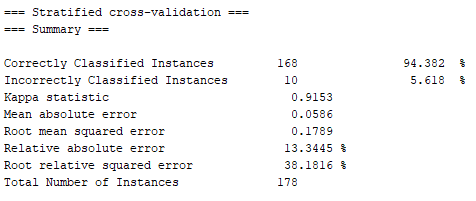
\includegraphics[width=\textwidth]{img/EGlobales.PNG}
    \caption{Estadísticas globales de nuestro clasificador}
\end{figure}

Nuestro clasificador ha realizado una muy buena clasificación obteniendo un total de 168 instancias bien clasificadas de las 178 totales con solo 10 erróneas.
Ha conseguido un 94.382\% de instancias bien clasificadas, frente a un 5.618\% de instancias mal clasificadas.

\begin{figure}[H]
    \centering
    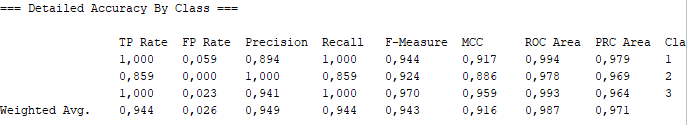
\includegraphics[width=\textwidth]{img/Ebyclass.PNG}
    \caption{Estadísticas de clasificación de cada clase}
\end{figure}

En la figura de arriba vemos una tabla en la cual nos da datos referentes a la clasificación más detallada de cada clase, cabe destacar los valores de TP Rate de la clase uno y dos(valores de uno para ambas clases) en  las cuales todas las instancias han sido clasificadas de manera correcta, además debemos de tener en cuenta la media de ROC Área que es muy cercana a uno la cual nos indica que nuestro clasificador está muy bien entrenado.

En la siguiente figura, la matriz de confusión, nos indica como se han clasificado las instancias en cada clase, vemos como lógicamente coincide con lo comentado anteriormente y en la clase a(1) y c(3) todas las instancias han sido clasificadas de manera correcta, mientras que en la clase b(2) de las 71 instancias pertenecientes a esta clase ha sido bien clasificadas 61, siendo de estas 7 clasificadas de manera errónea en la clase a(1) y 3 en la clase c(3).

\begin{figure}[H]
    \centering
    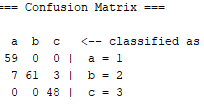
\includegraphics[width=0.9\textwidth]{img/MConf.PNG}
    \caption{Estadísticas de clasificación de cada clase}
\end{figure}


\subsection{Algoritmo Simple Logistic}
Con la base de datos escogida anteriormente, ejecute el algoritmo SimpleLogistic con 10-fold crossvalidation. 


\begin{figure}[H]
    \centering
    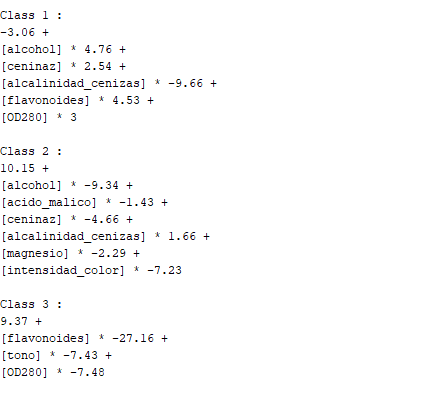
\includegraphics[width=\textwidth]{img/SL.PNG}
    \caption{Modelo de Regresión Logística obtenido al aplicar SampleLogistic}
    \label{fig:Modeloregresion}
\end{figure}
    
Una vez cargada nuestra base de datos Wine en Weka y preprocesada correctamente entramos en el apartado Classify para aplicar el algoritmo de regresión SampleLogistic, para ello entramos dentro de la carpeta functions que se encuentra a su vez dentro de la carpeta clasifiers y seleccionamos nuestro algoritmo.
En el resultado obtenido tal y como se indica en la figura de abajo nos aparece las distintas rectas de regresión obtenidas por el modelo, a partir de estas rectas mediante la función softmax obtenemos la probabilidad de pertenencia de una instancia a una de las clases. Además observamos (Fig\ref{fig:Modeloregresion}) como hay algunos atributos que no aparecen en estas funciones por lo tanto no son de utilidad a la hora de clasificar una instancia, estos atributos son, fenolestotales, fenolesnoflavonoides, proantocianinas.


En las siguientes ecuaciones que indican las rectas de regresión de las distintas clases vemos los valores de beta los cuales indican la importancia de las variables.Todas siguen la siguiente ecuación:

A continuación se expone la recta de regresión de la clase uno donde vemos que las variables que mas influyen son alcalinidad\_cenizas y alcohol. $f_1(x,\theta)=-3.06+Alcohol\ast4.76+ceninaz\ast2.54+alcalinidad\_cenizas\ast-9.66+flavonoides\ast4.53+OD280\ast3$

La siguiente ecuación \ref{ecuacion} nos muestra la recta de regresión de la clase dos donde debemos destacar que las variables mas influyentes son intensidad\_color y alcohol.

\begin{equation}
	f_1(X,\hat{\theta}) = \beta_0 + \sum_{i=1}^{n} \hat{\beta_i}x_i
	\label{ecuacion}
\end{equation}


$ f_2(x,\theta)=10.15+Alcohol\ast9.34+ceninaz\ast-4.66+alcalinidadcenizas\ast1.66+acidomalico\ast-1.43+magnesio\ast-2.29+intensidadcolor\ast-7.23 $


Por último tenemos la ecuación de regresión de la clase tres en la que destaca la importancia de la variable flavonoides.

$ f_3(x,\theta)=9.37+Flavonoides\ast-27.16+tono\ast-7.43+OD280\ast-7.48 $

Con respecto a las métricas se tiene un CCR 95.5056 de un  frente 94.38 al de un que daba el algoritmo KNN. El estadístico kappa 0.932 es igual a que como en el caso anterior quiere decir que el modelo obtenido es muy superior que uno basado en el azar. Por otro lado los valores de TP rate por clase son 0.983, 0.901 y 1 que son bastante similares a los obtenidos anteriormente. 

\begin{figure}[H]
    \centering
    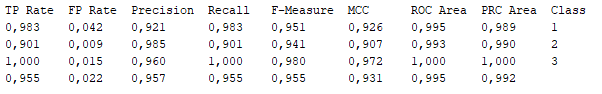
\includegraphics[width=\textwidth]{img/SLbyClass.PNG}
    \caption{Estadísticas de clasificación de cada clase}
    
\end{figure}
\chapter{Entregable 4}

\subsection{Ejercicio 1}

Escoja una de las bases de datos de clasificación para el trabajo de las dispuestas en Moodle. Se entiende que además de pasarla a formato .arff ya ha aplicado el preprocesamiento necesario en función del fichero "Pistas sobre los datasets con posible preprocesamiento a simple vista.pdf", en el caso que sea una de las bases de datos que lo requiera.

Cargue la base de datos y ejecute el algoritmo C4.5 usando un 75\% para entrenar y un 25\% para generalizar, con los parámetros por defecto.
Analice y muestre el árbol obtenido con los parámetros por defecto: nodo principal, número de nodos u hojas, variables presentes y omitidas. Comente también los resultados de las métricas obtenidas.

Para comenzar con el ejercicio hemos escogido la base de datos proporcionada por Moodle que anteriormente hemos pasado a formato .arff, esta base de datos consta de doce atributos de tipo numérico por lo cual deberíamos de aplicarle una discretización para así pasarlos a nominal, sin embargo esta es una de las ventajas del algoritmo empleado que a diferencia del algoritmo ID3 este, el C4.5 discretiza automáticamente por lo que para aplicarlo solo hemos tenido que modificar el tanto por ciento que deseamos destinar a entrenamiento tal y como muestra la figura de abajo.

\begin{figure}[H]
    \centering
    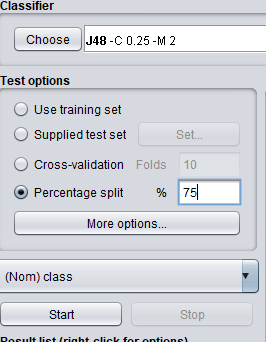
\includegraphics[width=\textwidth]{img/Porcentaje.PNG}
    \caption{Aplicación del 75\% de entrenamiento}
    
\end{figure}

A continuación mostraremos el árbol obtenido para comentar sus resultados así como sus reglas pertinentes y algunos datos de su estructura.

\begin{figure}[H]
    \centering
    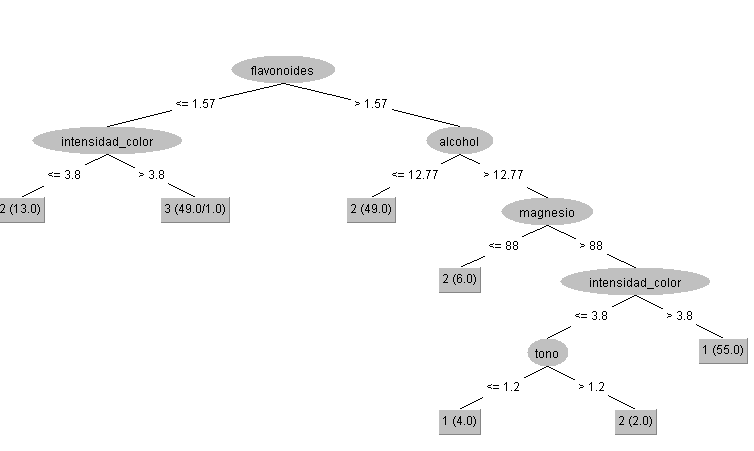
\includegraphics[width=\textwidth]{img/Tree.PNG}
    \caption{Árbol obtenido por el algoritmo C4.5}
    
\end{figure}

\begin{figure}[H]
    \centering
    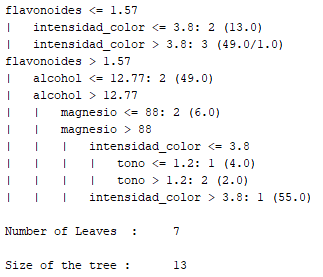
\includegraphics[width=\textwidth]{img/Reglas.PNG}
    \caption{Reglas propias del árbol}
    
\end{figure}

Cómo vemos en las figuras de arriba nuestro árbol está formado por seis nodos que corresponde con seis análisis de variable que son, flavonoides, intensidad\_color, alcohol, magnesio, y tono. Comenzamos analizando flavonoide ya que es esta la que nos produce una menor entropía. Además poseemos siete nodos terminales u hoja los cuales determinan a que clase pertenece la instancia analizada según el camino o reglas seguidas. También podemos destacar que hay alguna variables las cuales no aparecen lo que nos quiere decir que no son influyentes a la hora de clasificar una instancia, estas son, ácido\_malico, ceninaz, alcalinidad\_cenizas, fenoles\_totales, fenoles\_no\_flavonoides, proantocianinas y OD280.

Con respecto a las métricas debemos destacar un alto valor de CCR con un 93.1818\% además de un valor del estadístico Kappa de 0.8966 muy superior al 0.5 que representaría el azar. Con respecto a las métricas más especificas de cada clase debemos destacar un alto valor de TP Rate con valores de 0.882, 0.909 y 1 para cada clase respectivamente.
\begin{figure}[H]
    \centering
    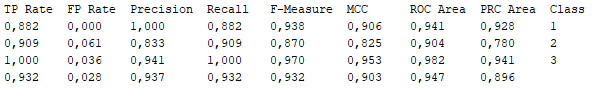
\includegraphics[width=\textwidth]{img/EC4.5.PNG}
    \caption{Estadísticas de clasificación de cada clase}
    
\end{figure}

Con ayuda de la matriz de confusión proporcionada por Weka vemos como de diecisiete instancias a clasificar de la clase a(1) quince han sido clasificadas bien frente a dos que han sido clasificadas de manera errónea en la clase b(2), con respecto a la clase b(2) vemos cómo de once instancias, diez han sido bien clasificadas frente a una que ha sido clasificada como de clase c(3), por último destacar que en la clase c(3) todas han sido bien clasificada haciendo un total de dieciséis.

A continuación se muestra la matriz de confusión para una mejor comprensión de lo anterior. 

\begin{figure}[H]
    \centering
    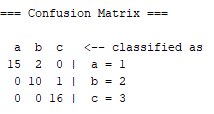
\includegraphics[width=\textwidth]{img/MC4.5.PNG}
    \caption{Estadísticas de clasificación de cada clase}
\end{figure}

\subsection{Ejercicio 2}

Escoja una de las bases de datos de clasificación para el trabajo de las dispuestas en Moodle. Se entiende que además de pasarla a formato .arff ya ha aplicado el preprocesamiento necesario en función del fichero "Pistas sobre los datasets con posible preprocesamiento a simple vista.pdf", en el caso que sea una de las bases de datos que lo requiera.
Cargue la base de datos con un 75/25\% y ejecute el algoritmo MultilayerPerceptron con los valores por defecto.
¿Qué observa al ir modificando solo el TrainingTime? ¿Cambia el valor de Correctly Classified instances al modificar el parámetro? ¿se estanca el aprendizaje o sobre entrena?
¿Qué observa al ir modificando solo el LeraningRate? ¿Cambia el valor de Correctly Classified instances al modificar el parámetro? ¿se estanca el aprendizaje o sobre entrena?

Para realizar este ejercicio hemos escogido la base de datos wine.arff utilizada con anteriores ejemplos.
De manera inicial con todos los valores por defecto y con un valor para TrainingTime de 500 tal y como viene por defecto el algoritmo nos clasifica 43 de las 44 destinadas a prueba de manera correcta, a medida que aumentamos el TrainingTime el valor del CCR sigue constante por lo que el algoritmo se estanca, por tanto hemos optado por reducirlo a la unidad e ir incrementando hasta comprobar donde este algoritmo de estanca que ha sido en un valor de siete. En la figura de abajo se muestra con más claridad la evolución del CCR.
\begin{figure}[H]
    \centering
    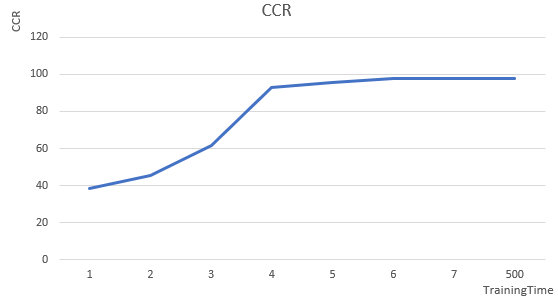
\includegraphics[width=\textwidth]{img/GM.PNG}
    \caption{Evolución del CCR con respecto a TrainingTime}

\end{figure}
 --------------------------------------------------------------

% BIBLIOGRAFIA --------------------------------------------------------------------------
% Localizacion de Bibliografía .bib para BibTex
\backmatter
%\printbibliography[heading=bibintoc, title={Bibliografía}]
\bibliographystyle{plain}
\bibliography{./Practicas/bibliografia}
%Necesario para que imprima toda la bibliografia sin hacer falta ser referenciada en el texto
\nocite{*}
 -----------------------------------------------------------------------
\end{document}